\documentclass[border=8pt,tikz]{standalone}
\usepackage[utf8]{inputenc}
\usepackage[T1]{fontenc}
\usepackage{helvet}
\renewcommand{\familydefault}{\sfdefault}
\usepackage{tikz}
\usetikzlibrary{positioning, shapes.multipart, arrows.meta}

\definecolor{factColor}{HTML}{7F77DD}
\definecolor{factBorder}{HTML}{3C3489}
\definecolor{dimColor}{HTML}{9FE1CB}
\definecolor{dimBorder}{HTML}{0F6E56}
\definecolor{headerColor}{HTML}{534AB7}
\definecolor{dimHeader}{HTML}{1D9E75}
\definecolor{textDark}{HTML}{2C2C2A}

\begin{document}

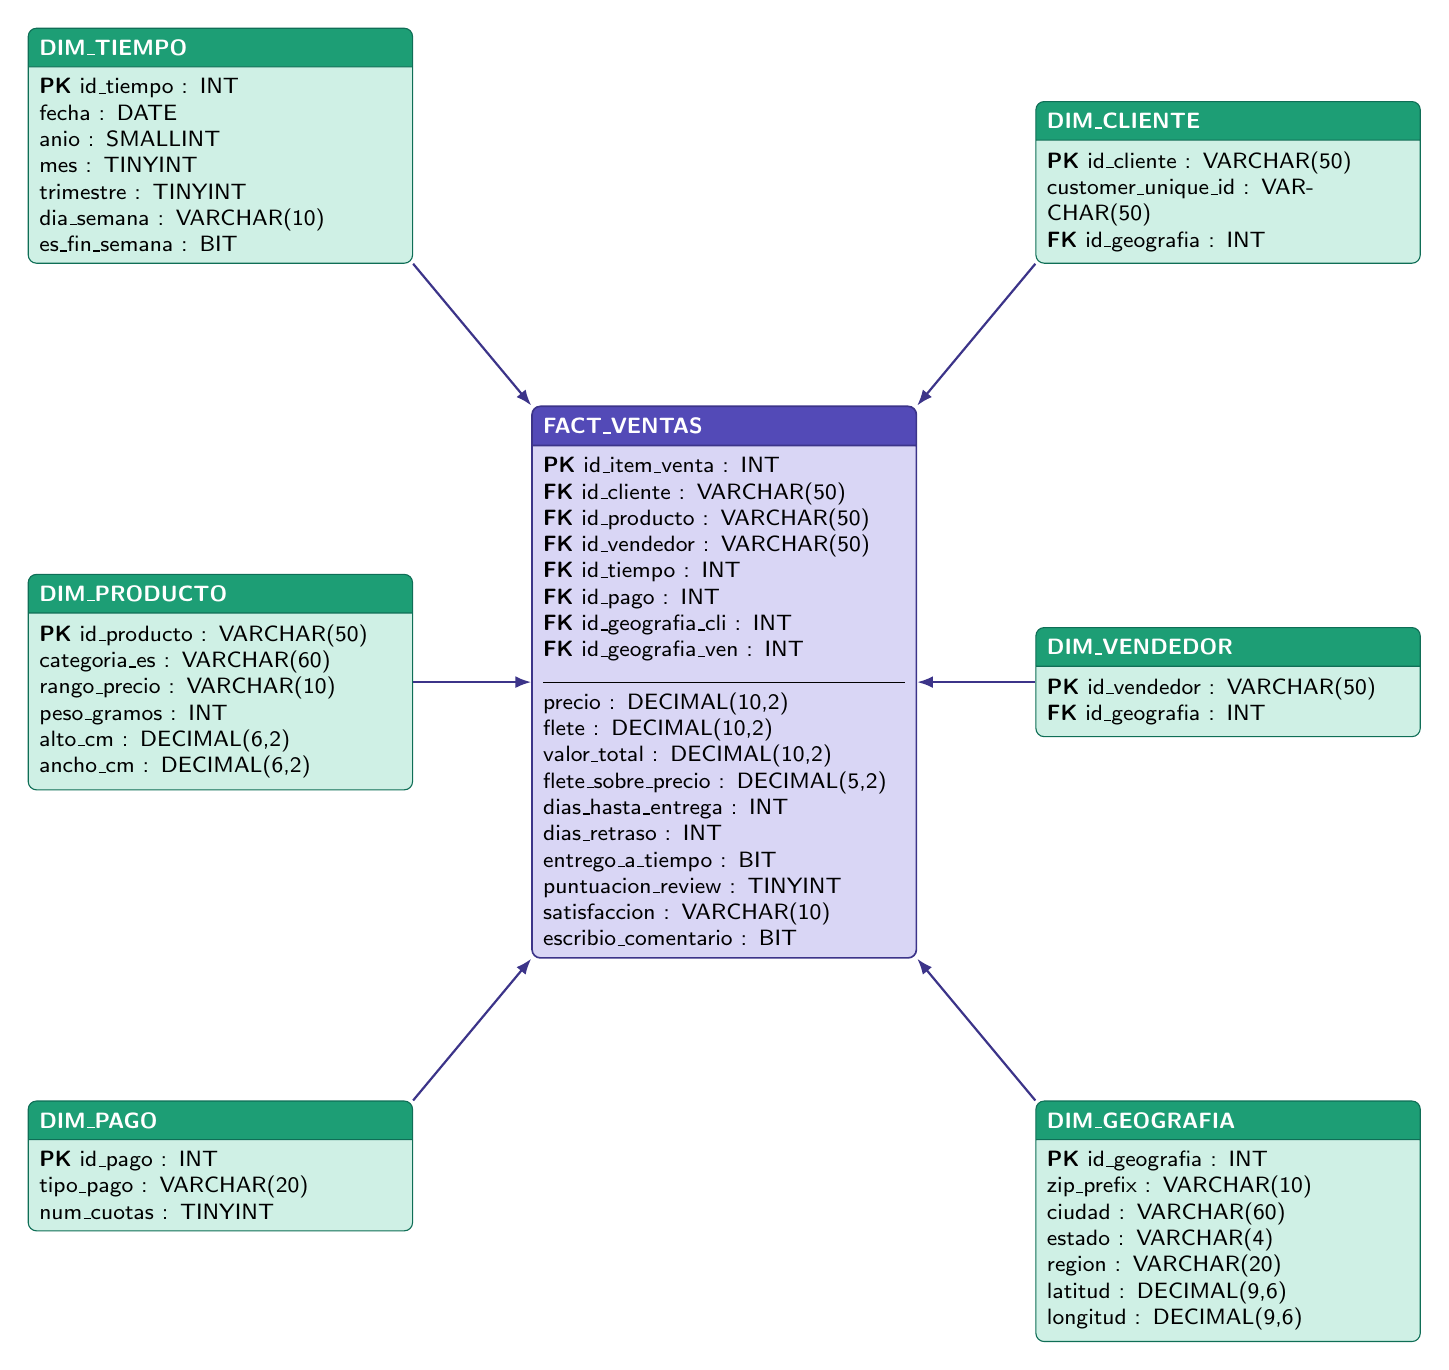
\begin{tikzpicture}[
    every node/.style={font=\footnotesize},
    tablestyle/.style={
        rectangle split,
        rectangle split parts=2,
        draw,
        line width=0.4pt,
        rounded corners=3pt,
        inner sep=4pt,
        text width=4.6cm,
        align=left,
    },
    fact/.style={
        tablestyle,
        rectangle split part fill={headerColor, factColor!30},
        draw=factBorder,
        line width=0.6pt,
    },
    dim/.style={
        tablestyle,
        rectangle split part fill={dimHeader, dimColor!50},
        draw=dimBorder,
    },
    header/.style={
        text=white,
        font=\footnotesize\bfseries,
    },
    rel/.style={
        -{Latex[length=2mm, width=1.5mm]},
        thick,
        color=factBorder,
    },
]

\node[fact] (fact) at (0,0) {
    \nodepart{one}\textcolor{white}{\textbf{FACT\_VENTAS}}
    \nodepart{two}
    \textbf{PK} id\_item\_venta : INT\\
    \textbf{FK} id\_cliente : VARCHAR(50)\\
    \textbf{FK} id\_producto : VARCHAR(50)\\
    \textbf{FK} id\_vendedor : VARCHAR(50)\\
    \textbf{FK} id\_tiempo : INT\\
    \textbf{FK} id\_pago : INT\\
    \textbf{FK} id\_geografia\_cli : INT\\
    \textbf{FK} id\_geografia\_ven : INT\\
    \hrulefill\\
    precio : DECIMAL(10,2)\\
    flete : DECIMAL(10,2)\\
    valor\_total : DECIMAL(10,2)\\
    flete\_sobre\_precio : DECIMAL(5,2)\\
    dias\_hasta\_entrega : INT\\
    dias\_retraso : INT\\
    entrego\_a\_tiempo : BIT\\
    puntuacion\_review : TINYINT\\
    satisfaccion : VARCHAR(10)\\
    escribio\_comentario : BIT
};

\node[dim, above left=1.8cm and 1.5cm of fact] (tiempo) {
    \nodepart{one}\textcolor{white}{\textbf{DIM\_TIEMPO}}
    \nodepart{two}
    \textbf{PK} id\_tiempo : INT\\
    fecha : DATE\\
    anio : SMALLINT\\
    mes : TINYINT\\
    trimestre : TINYINT\\
    dia\_semana : VARCHAR(10)\\
    es\_fin\_semana : BIT
};

\node[dim, above right=1.8cm and 1.5cm of fact] (cliente) {
    \nodepart{one}\textcolor{white}{\textbf{DIM\_CLIENTE}}
    \nodepart{two}
    \textbf{PK} id\_cliente : VARCHAR(50)\\
    customer\_unique\_id : VARCHAR(50)\\
    \textbf{FK} id\_geografia : INT
};

\node[dim, left=1.5cm of fact] (producto) {
    \nodepart{one}\textcolor{white}{\textbf{DIM\_PRODUCTO}}
    \nodepart{two}
    \textbf{PK} id\_producto : VARCHAR(50)\\
    categoria\_es : VARCHAR(60)\\
    rango\_precio : VARCHAR(10)\\
    peso\_gramos : INT\\
    alto\_cm : DECIMAL(6,2)\\
    ancho\_cm : DECIMAL(6,2)
};

\node[dim, right=1.5cm of fact] (vendedor) {
    \nodepart{one}\textcolor{white}{\textbf{DIM\_VENDEDOR}}
    \nodepart{two}
    \textbf{PK} id\_vendedor : VARCHAR(50)\\
    \textbf{FK} id\_geografia : INT
};

\node[dim, below left=1.8cm and 1.5cm of fact] (pago) {
    \nodepart{one}\textcolor{white}{\textbf{DIM\_PAGO}}
    \nodepart{two}
    \textbf{PK} id\_pago : INT\\
    tipo\_pago : VARCHAR(20)\\
    num\_cuotas : TINYINT
};

\node[dim, below right=1.8cm and 1.5cm of fact] (geografia) {
    \nodepart{one}\textcolor{white}{\textbf{DIM\_GEOGRAFIA}}
    \nodepart{two}
    \textbf{PK} id\_geografia : INT\\
    zip\_prefix : VARCHAR(10)\\
    ciudad : VARCHAR(60)\\
    estado : VARCHAR(4)\\
    region : VARCHAR(20)\\
    latitud : DECIMAL(9,6)\\
    longitud : DECIMAL(9,6)
};

\draw[rel] (tiempo.south east) -- (fact.north west);
\draw[rel] (cliente.south west) -- (fact.north east);
\draw[rel] (producto.east) -- (fact.west);
\draw[rel] (vendedor.west) -- (fact.east);
\draw[rel] (pago.north east) -- (fact.south west);
\draw[rel] (geografia.north west) -- (fact.south east);

\end{tikzpicture}

\end{document}
